\documentclass{article}
\usepackage[export]{adjustbox}
\usepackage[utf8]{inputenc}
\usepackage[section]{placeins}
\usepackage[french]{babel}
\usepackage[T1]{fontenc}
\usepackage[top=60pt, bottom=60pt]{geometry}

\title{Effets des mesures liées à la Covid-19 sur les liens de collaboration entre les étudiants en écologie de l'université Sherbrooke}
\author{William Jacques, Olivier Kaprolat, Guillaume Tougas \\ et Nicolas Vachon}
\date{25 avril 2021}

\begin{document}

\maketitle

\begin{abstract}
Dans cette étude, nous analysons l'effet de la pandémie de la Covid-19 sur le type de cours donné, soit en ligne ou en présentiel, ainsi que sur l'appariement entre les étudiants participant au cours BIO500 à l'université de Sherbrooke à l'hiver 2021 en ce qui a trait à leurs travaux d'équipe. Pour ce faire, les données rapportées par plusieurs sous-groupes d'étudiants ont été utilisées afin de générer des figures comparant les collaborations pré et post-Covid. Nous avons d'abord illustré qu'il y a davantage de cours en ligne pour la période post-Covid. Toutefois, nous n'avons pas été en mesure de confirmer nos hypothèses supposant que la diversité des équipes devrait diminuer et que les étudiants seraient plus conservateurs dans le choix de leurs coéquipiers en période post-Covid et dans les cours en ligne.
\end{abstract}

\section{Introduction}
En ces temps pandémiques et maussades, l’ensemble de la population est affectée par des changements drastiques de mode de vie nécessaires pour diminuer la propagation du virus et de ses variants. Ainsi, on observe une dégradation majeure de la santé mentale chez les étudiants depuis le début des mesures sanitaires liées à la Covid-19 \cite{son_effects_2020}. En effet, on note une augmentation du stress, de l’anxiété et des pensées dépressives chez ceux-ci. Toutefois, depuis le confinement, il semble que leur performance académique se soit améliorée, puisque les distractions ont diminué, ce qui leur aurait permis de développer des méthodes d'étude plus efficaces \cite{gonzalez_influence_2020}. Une chose est certaine: les mesures liées à la Covid-19 ont un important effet sur les étudiants, particulièrement sur leur comportement. Dans cette étude, nous nous intéressons d’ailleurs à l’impact de ces mesures sur la dynamique de la formation des équipes dans le cadre de travaux scolaires. Plus précisément, nous nous intéressons à l’effet des mesures liées à la Covid-19 sur le nombre de cours en ligne et les collaborations entre les étudiants. Selon nous, il devrait y avoir davantage de cours en ligne et la diversité des équipes devrait diminuer en période de pandémie. De plus, nous estimons que les étudiants sont plus conservateurs dans leur choix de coéquipier depuis le début de la pandémie ainsi que dans les cours en ligne, comparativement à la période pré-Covid et dans les cours en présentiel. 

\section{Méthodes} Tout d'abord, les données proviennent de nombreux sous-groupes d'étudiants qui ont fait l'inventaire des collaborations auxquelles ils ont participé jusqu'à présent dans le cadre de leur baccalauréat en biologie à l'Université de Sherbrooke. Ils ont aussi recensé diverses informations sur les collaborateurs : leur session de début de baccalauréat, leur programme d'étude, s'ils sont en régime coop ainsi que leur participation actuelle au cours BIO500 ou pas. Ils ont également noté des informations sur leurs collaborations : l'identité des personnes y ayant pris part, le cours dans lequel la collaboration a eu lieu ainsi que la date de celle-ci. Enfin, ils ont recensé des informations sur les cours dans lesquels les collaborations ont eu lieu : le sigle du cours, le nombre de crédits associé à ce cours, s'il est en présentiel ou en ligne et si les équipes pour les travaux de ce cours étaient choisies librement. D'ailleurs, il est à noter que les données considérées proviennent de sous-groupes d'étudiants appartenant seulement à la moitié du groupe du cours BIO500. Ensuite, il a été nécessaire d'effectuer certaines modifications sur les données compilées afin de les réconcilier entre elles et de les combiner en une seule base de données. Afin de s'assurer que le tout soit reproductible, les modifications ont été réalisées à même un script sur le logiciel R et elles ont été annotées. Suite à leur fusion en fichiers de données englobant toutes les équipes, nous avons sélectionné certaines données spécifiques provenant de notre base de données SQL à l'aide de requêtes dans le but de générer des tableaux et figures pertinents. Le package SQLite s'est avéré nécessaire à cet effet. Toujours à des fins de reproductibilité, les bases de données brutes ainsi que l'entièreté des scripts utilisés pour effectuer l'analyse et les figures ont été téléversés sur une version en ligne du système de contrôle de versions Git appelée GitHub.
\section{Résultats}
Dans le tableau 1, nous remarquons que la moyenne de collaborations pour un étudiant est plus élevée durant la période pré-Covid que durant la période post-Covid. Dans la figure 1, il est possible d'observer l'évolution du réseau de collaboration entre les périodes pré et post-Covid. Le réseau semble d'ailleurs moins diversifié dans la période post-Covid. Dans la figure 2, on peut voir que les proportions du nombre de fois où il y a eu collaboration entre les deux mêmes personnes ne semble pas différer significativement entre les périodes pré et post-Covid. Dans la figure 3, on observe qu'il y a beaucoup plus de cours en ligne en période post-Covid que pré-Covid. Dans la figure 4, la seule différence notable est que dans les cours en présentiel, il y a une proportion plus élevée de grands nombres de collaborations entre deux étudiants.
\clearpage
\begin{table}[h!]
\centering

\begin{center}
\begin{tabular}{|c|p{3cm}|p{3cm}|}

\hline
Étudiants & Nombre de collaborations pré-covid & Nombre de collaborations post-covid\\
\hline
arhire\_elizarebecca & 9 & 2\\
\hline
auger\_laurent & 9 & 5\\
\hline
beauregard\_crystel & 8 & 5\\
\hline
bernier\_raphael & 10 & 6\\
\hline
blanchard\_sebastien & 21 & 12\\
\hline
boulerice\_laurie & 10 & 11\\
\hline
caya\_anthony & 7 & 4\\
\hline
chaput\_lydia & 1 & 6\\
\hline
cloutier\_benjamin & 17 & 5\\
\hline
cloutier\_zachary & 3 & 4\\
\hline
coursol\_denver & 10 & 8\\
\hline
cyr\_marcantoine & 7 & 4\\
\hline
dagenaisquesnel\_benjamin & 13 & 9\\
\hline
deblois\_fanny & 7 & 6\\
\hline
fortier\_catherine & 8 & 5\\
\hline
godon\_coralie & 12 & 4\\
\hline
jacques\_william & 10 & 9\\
\hline
kaprolat\_olivier & 11 & 14\\
\hline
laberge\_anneju & 13 & 4\\
\hline
lapointe\_eve & 7 & 6\\
\hline
leduc\_francoisxavier & 7 & 2\\
\hline
lesperance\_laurie & 11 & 3\\
\hline
luangphachaleun\_arigna & 6 & 6\\
\hline
meriel\_clara & 8 & 5\\
\hline
merineau\_ariane & 9 & 5\\
\hline
michaudleblanc\_esther & 6 & 5\\
\hline
nappertdrouin\_anais & 10 & 4\\
\hline
normandboisseau\_florence & 9 & 1\\
\hline
ouellet\_laury & 9 & 3\\
\hline
tougas\_guillaume & 12 & 6\\
\hline
vachon\_nicolas & 13 & 5\\
\hline
vincent\_william & 6 & 8\\
\hline
vinet\_tanya & 16 & 18\\
\hline
whitter\_olivier & 9 & 5\\
\hline
Moyenne de collaboration par étudiant & 8,94 & 5,97 \\
\hline
\end{tabular}
\end{center}

\caption{Nombre de collaborations total par personne dans les périodes pré et post-Covid.}
\end{table}

 \begin{figure}[bp!]
\centerline{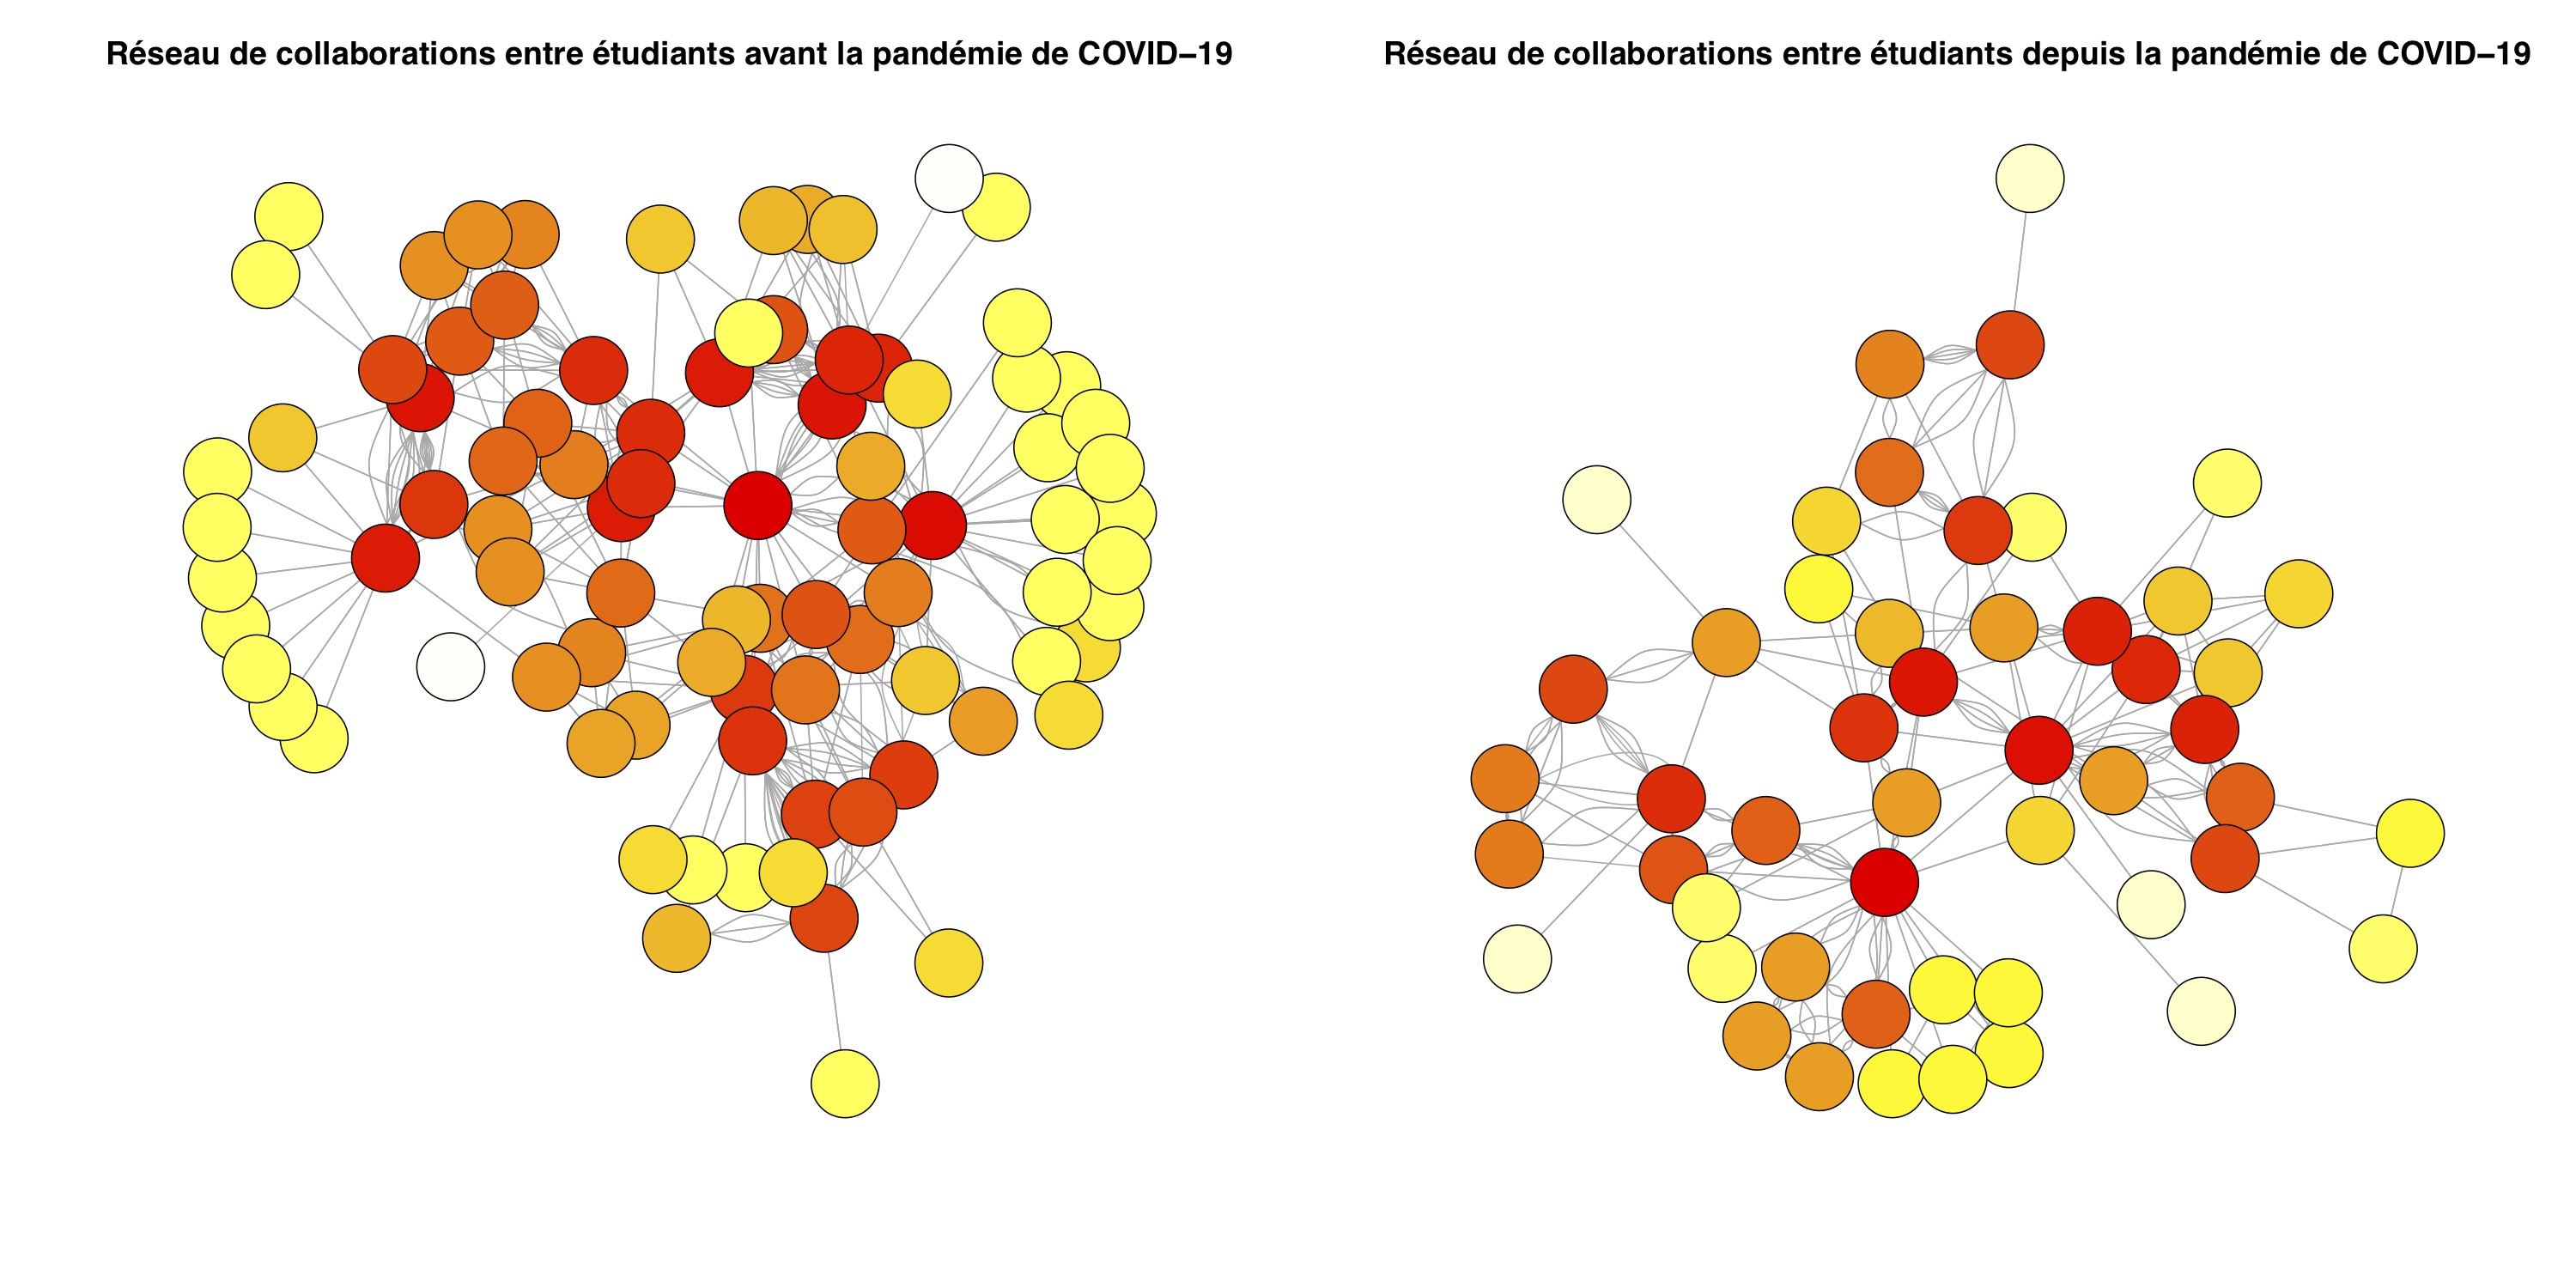
\includegraphics[scale=0.15]{Reseau_comparaison.jpg}}
\caption{Comparaison visuelle des réseaux de collaboration pré et post-Covid. Les cercles du plus rouge au plus blanc représentent respectivement les personnes avec le plus de collaborations aux personnes avec le moins de collaborations. }
\label{fig}
\end{figure}
 \begin{figure}[bp!]
\centerline{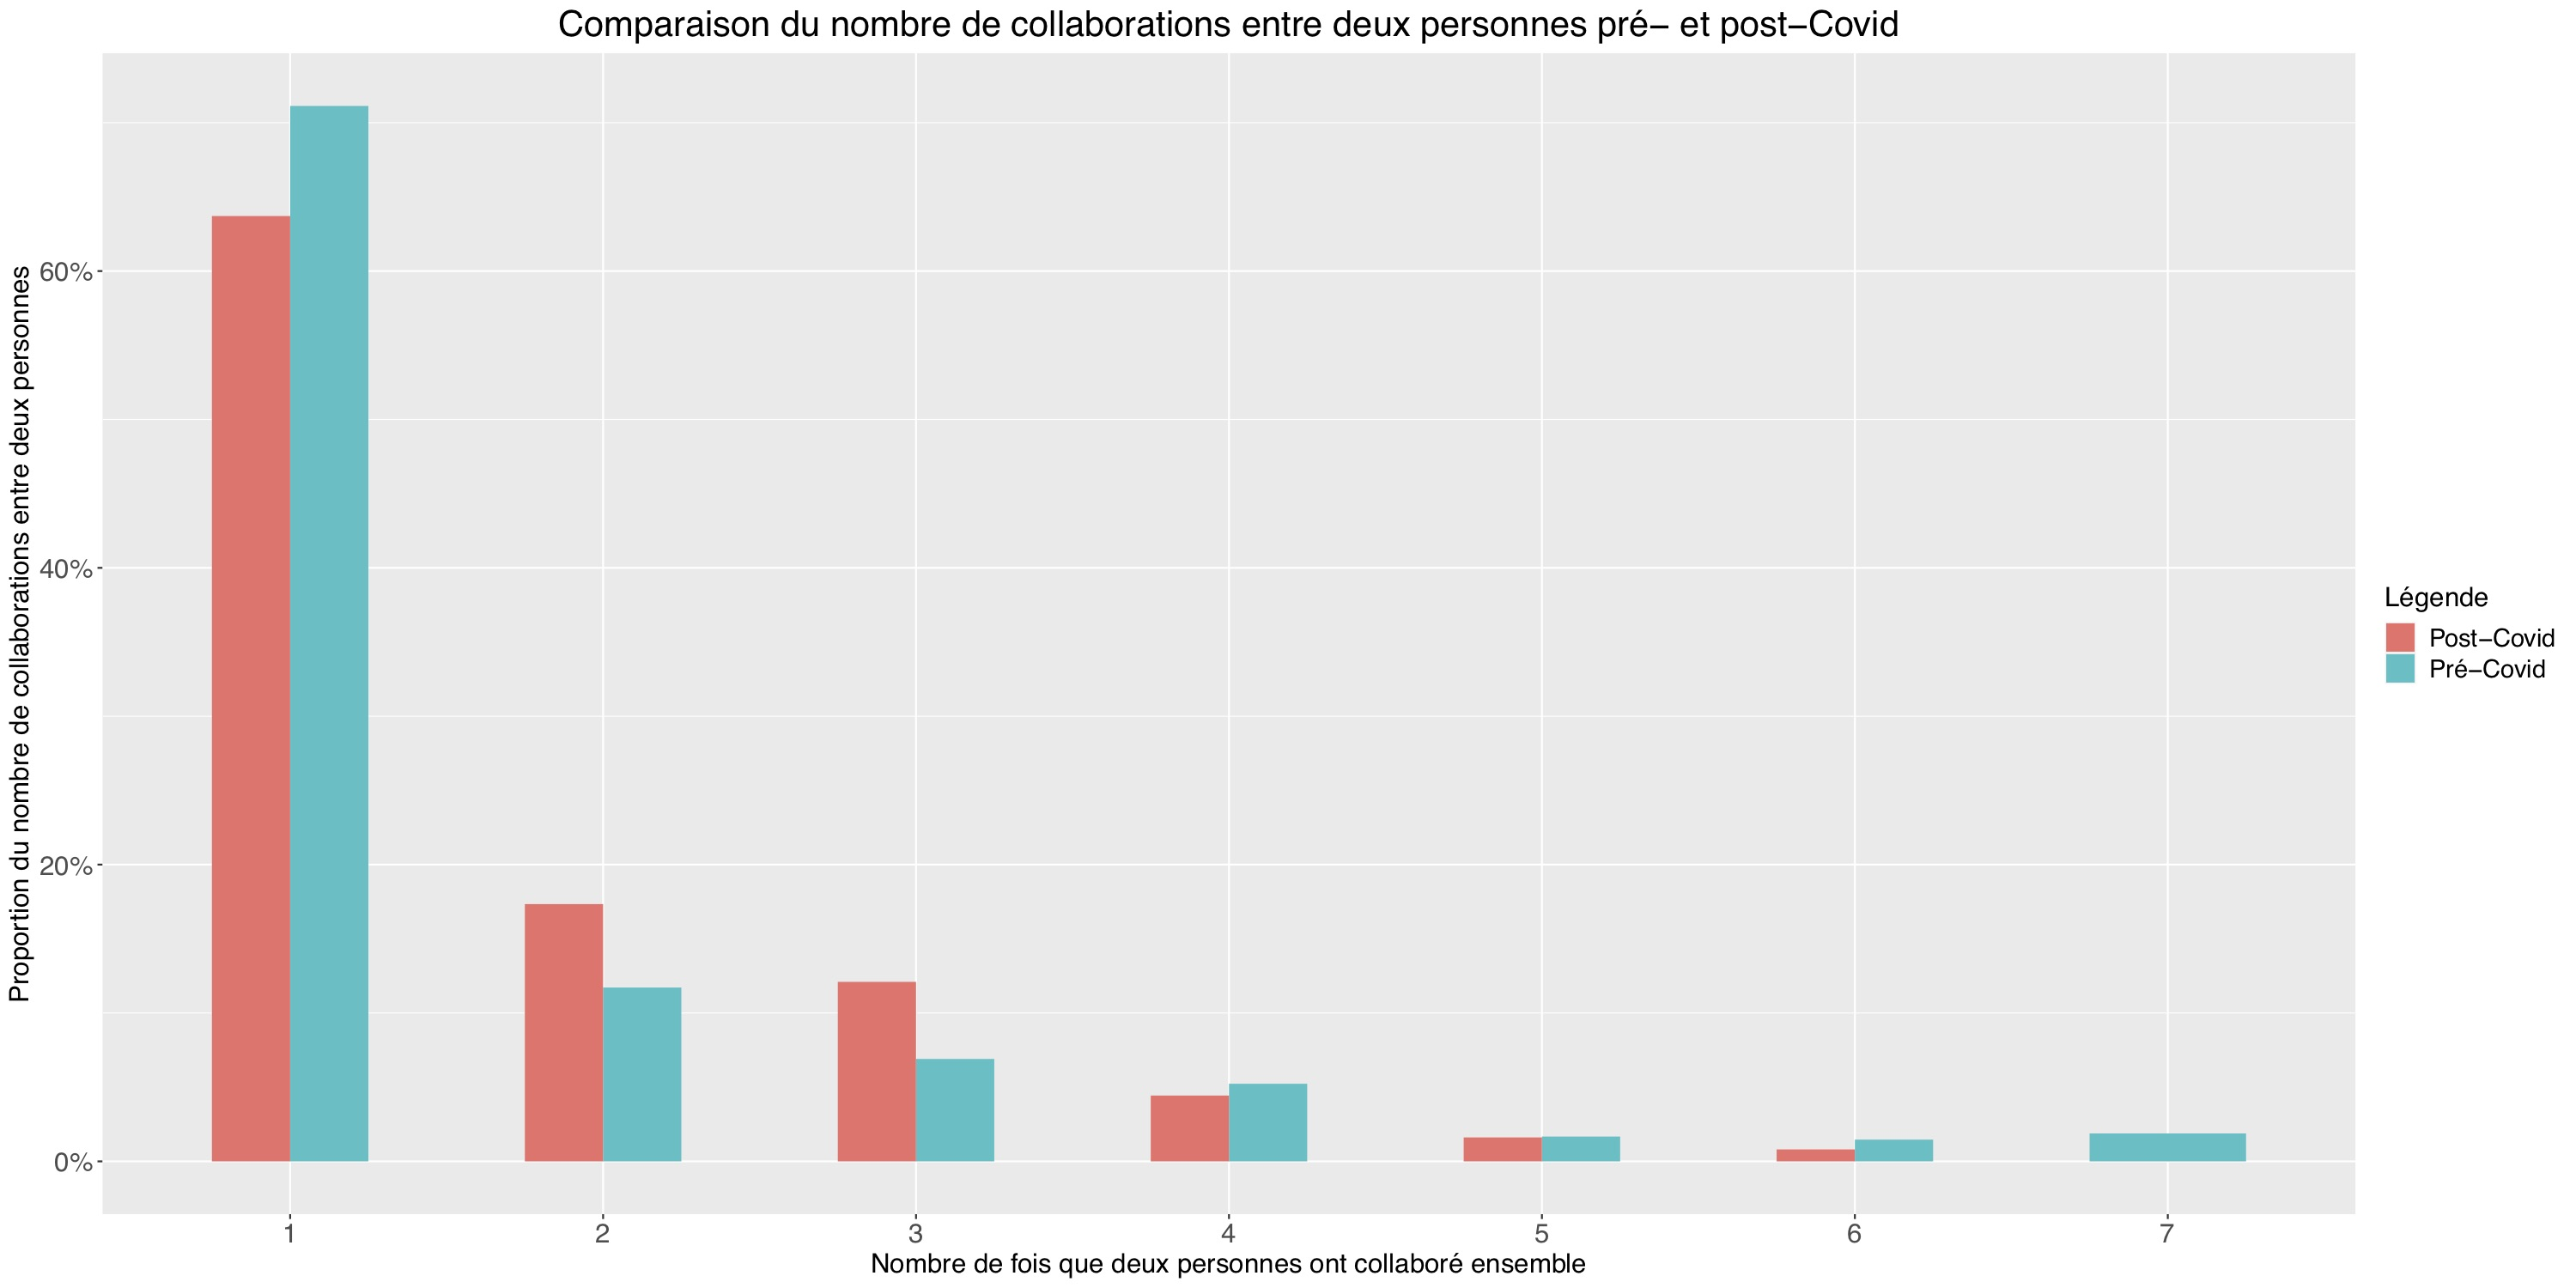
\includegraphics[scale=0.15]{Histogramme2.jpg}}
\caption{Histogramme de comparaison des différences dans les proportions du nombre de fois où il y a eu collaboration avec la même personne entre les périodes pré et post-Covid.}
\label{fig}
\end{figure}

 \begin{figure}[bp!]
\centerline{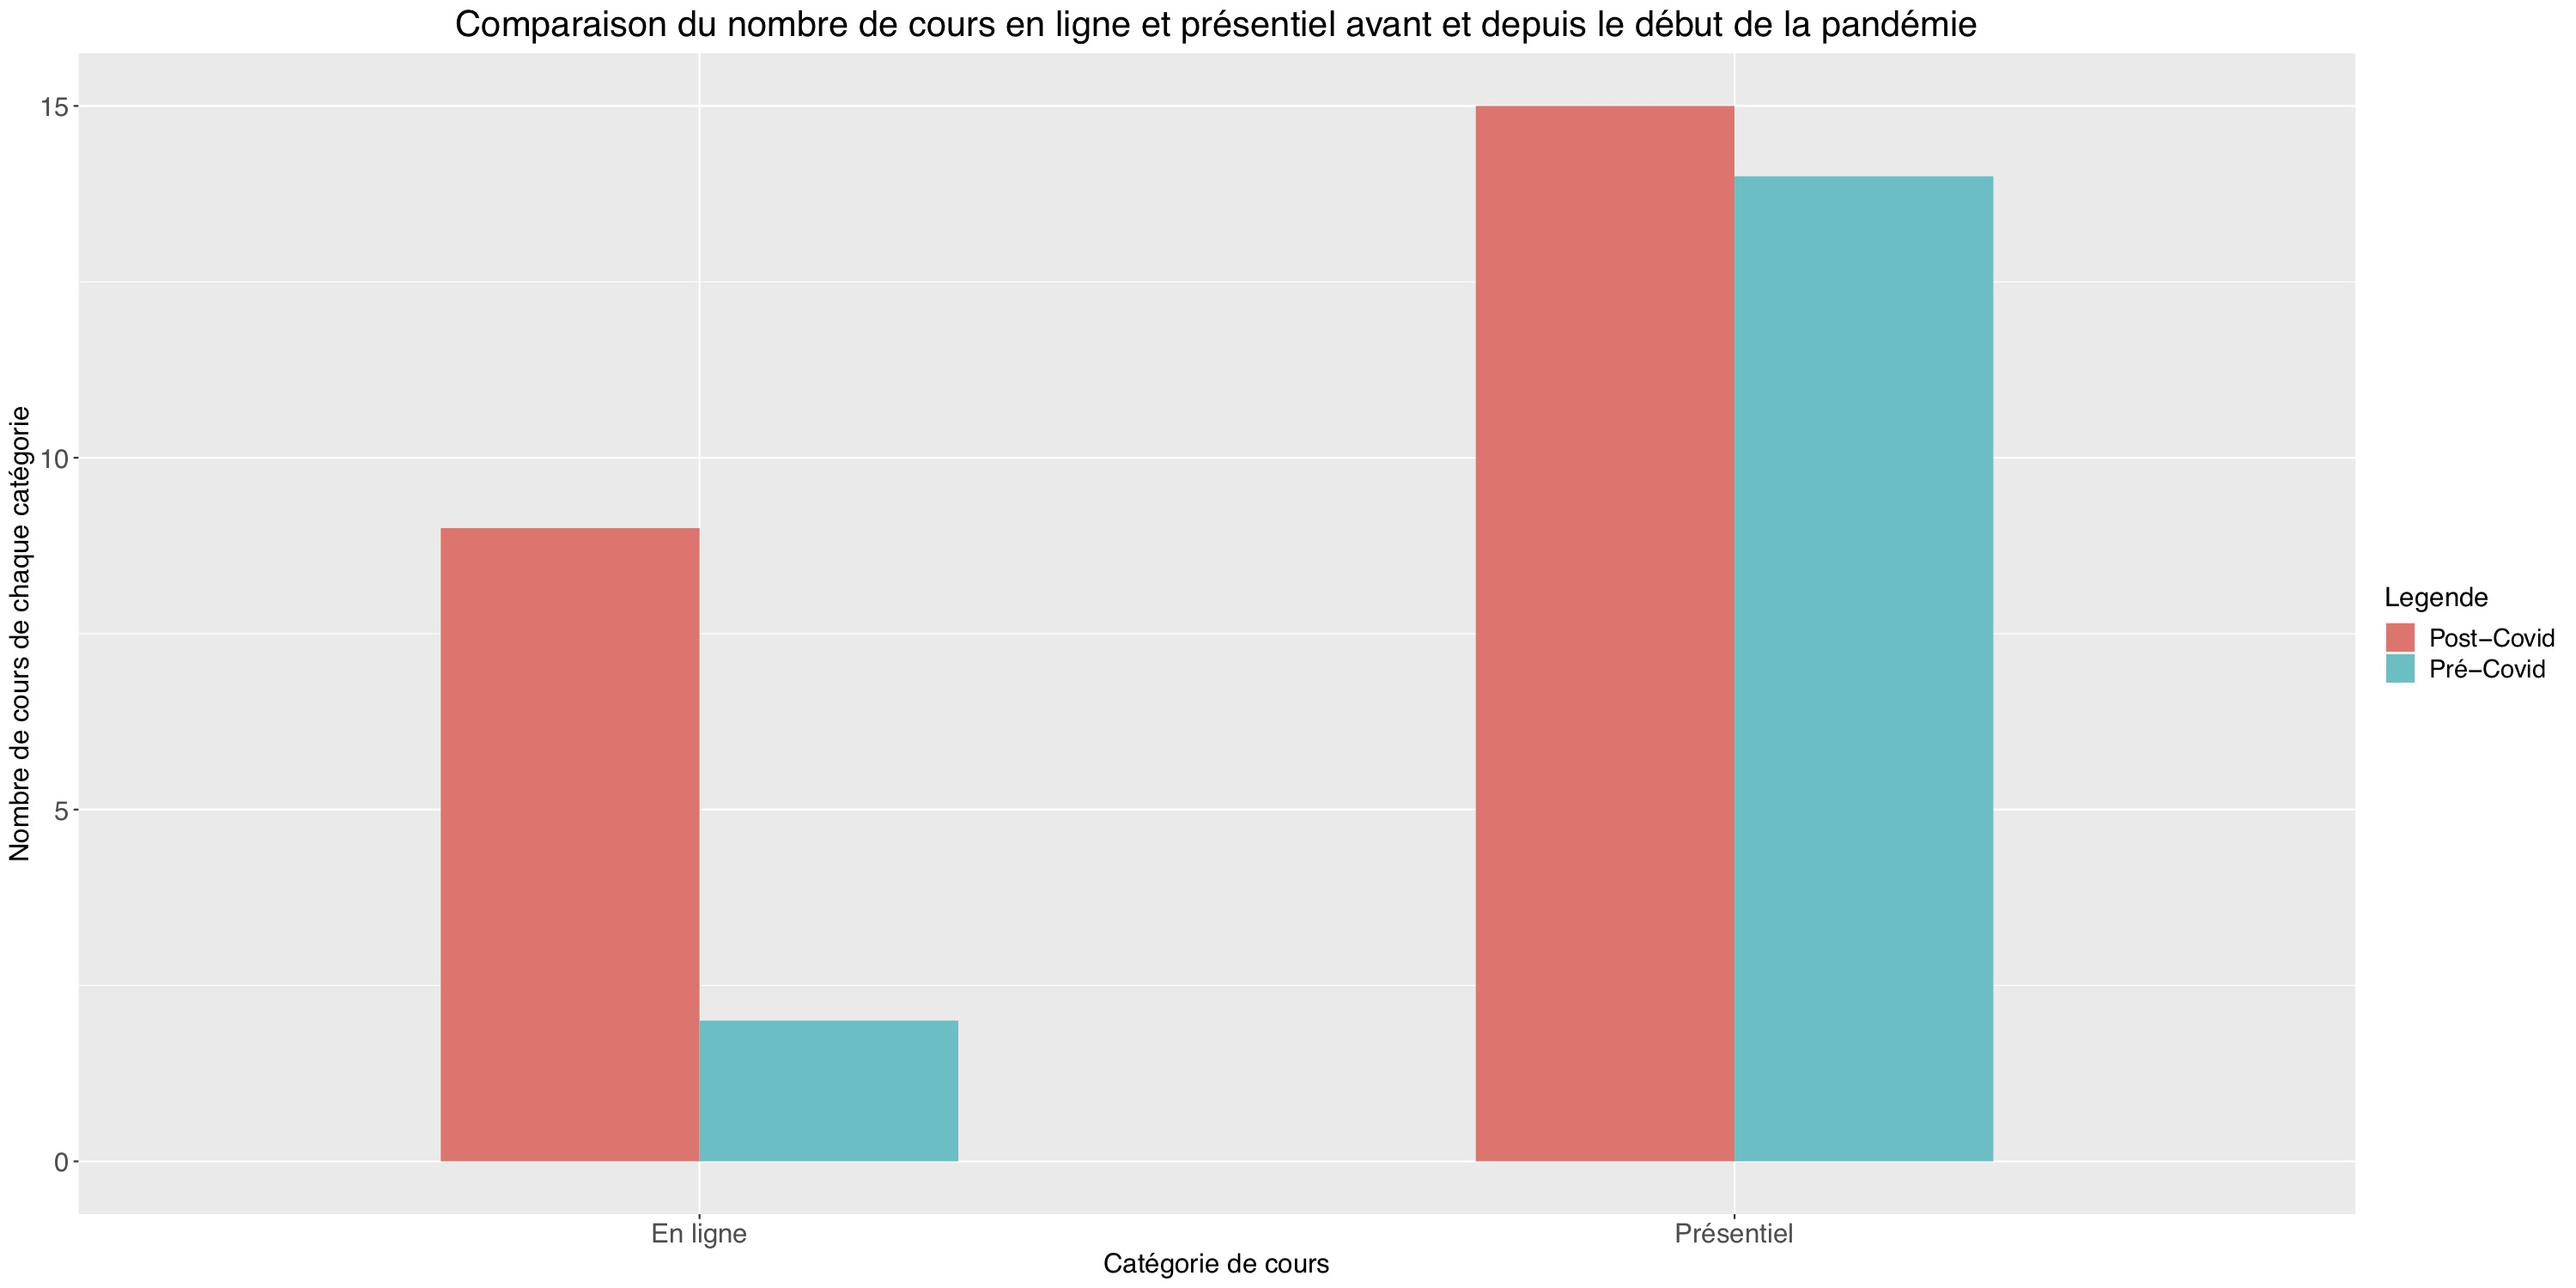
\includegraphics[scale=0.15]{Histogramme4.jpg}}
\caption{Histogramme de comparaison du nombre de cours en ligne et en présentiel en période pré et post-Covid.}
\label{fig}
\end{figure}
 
 \begin{figure}[bp!]
\centerline{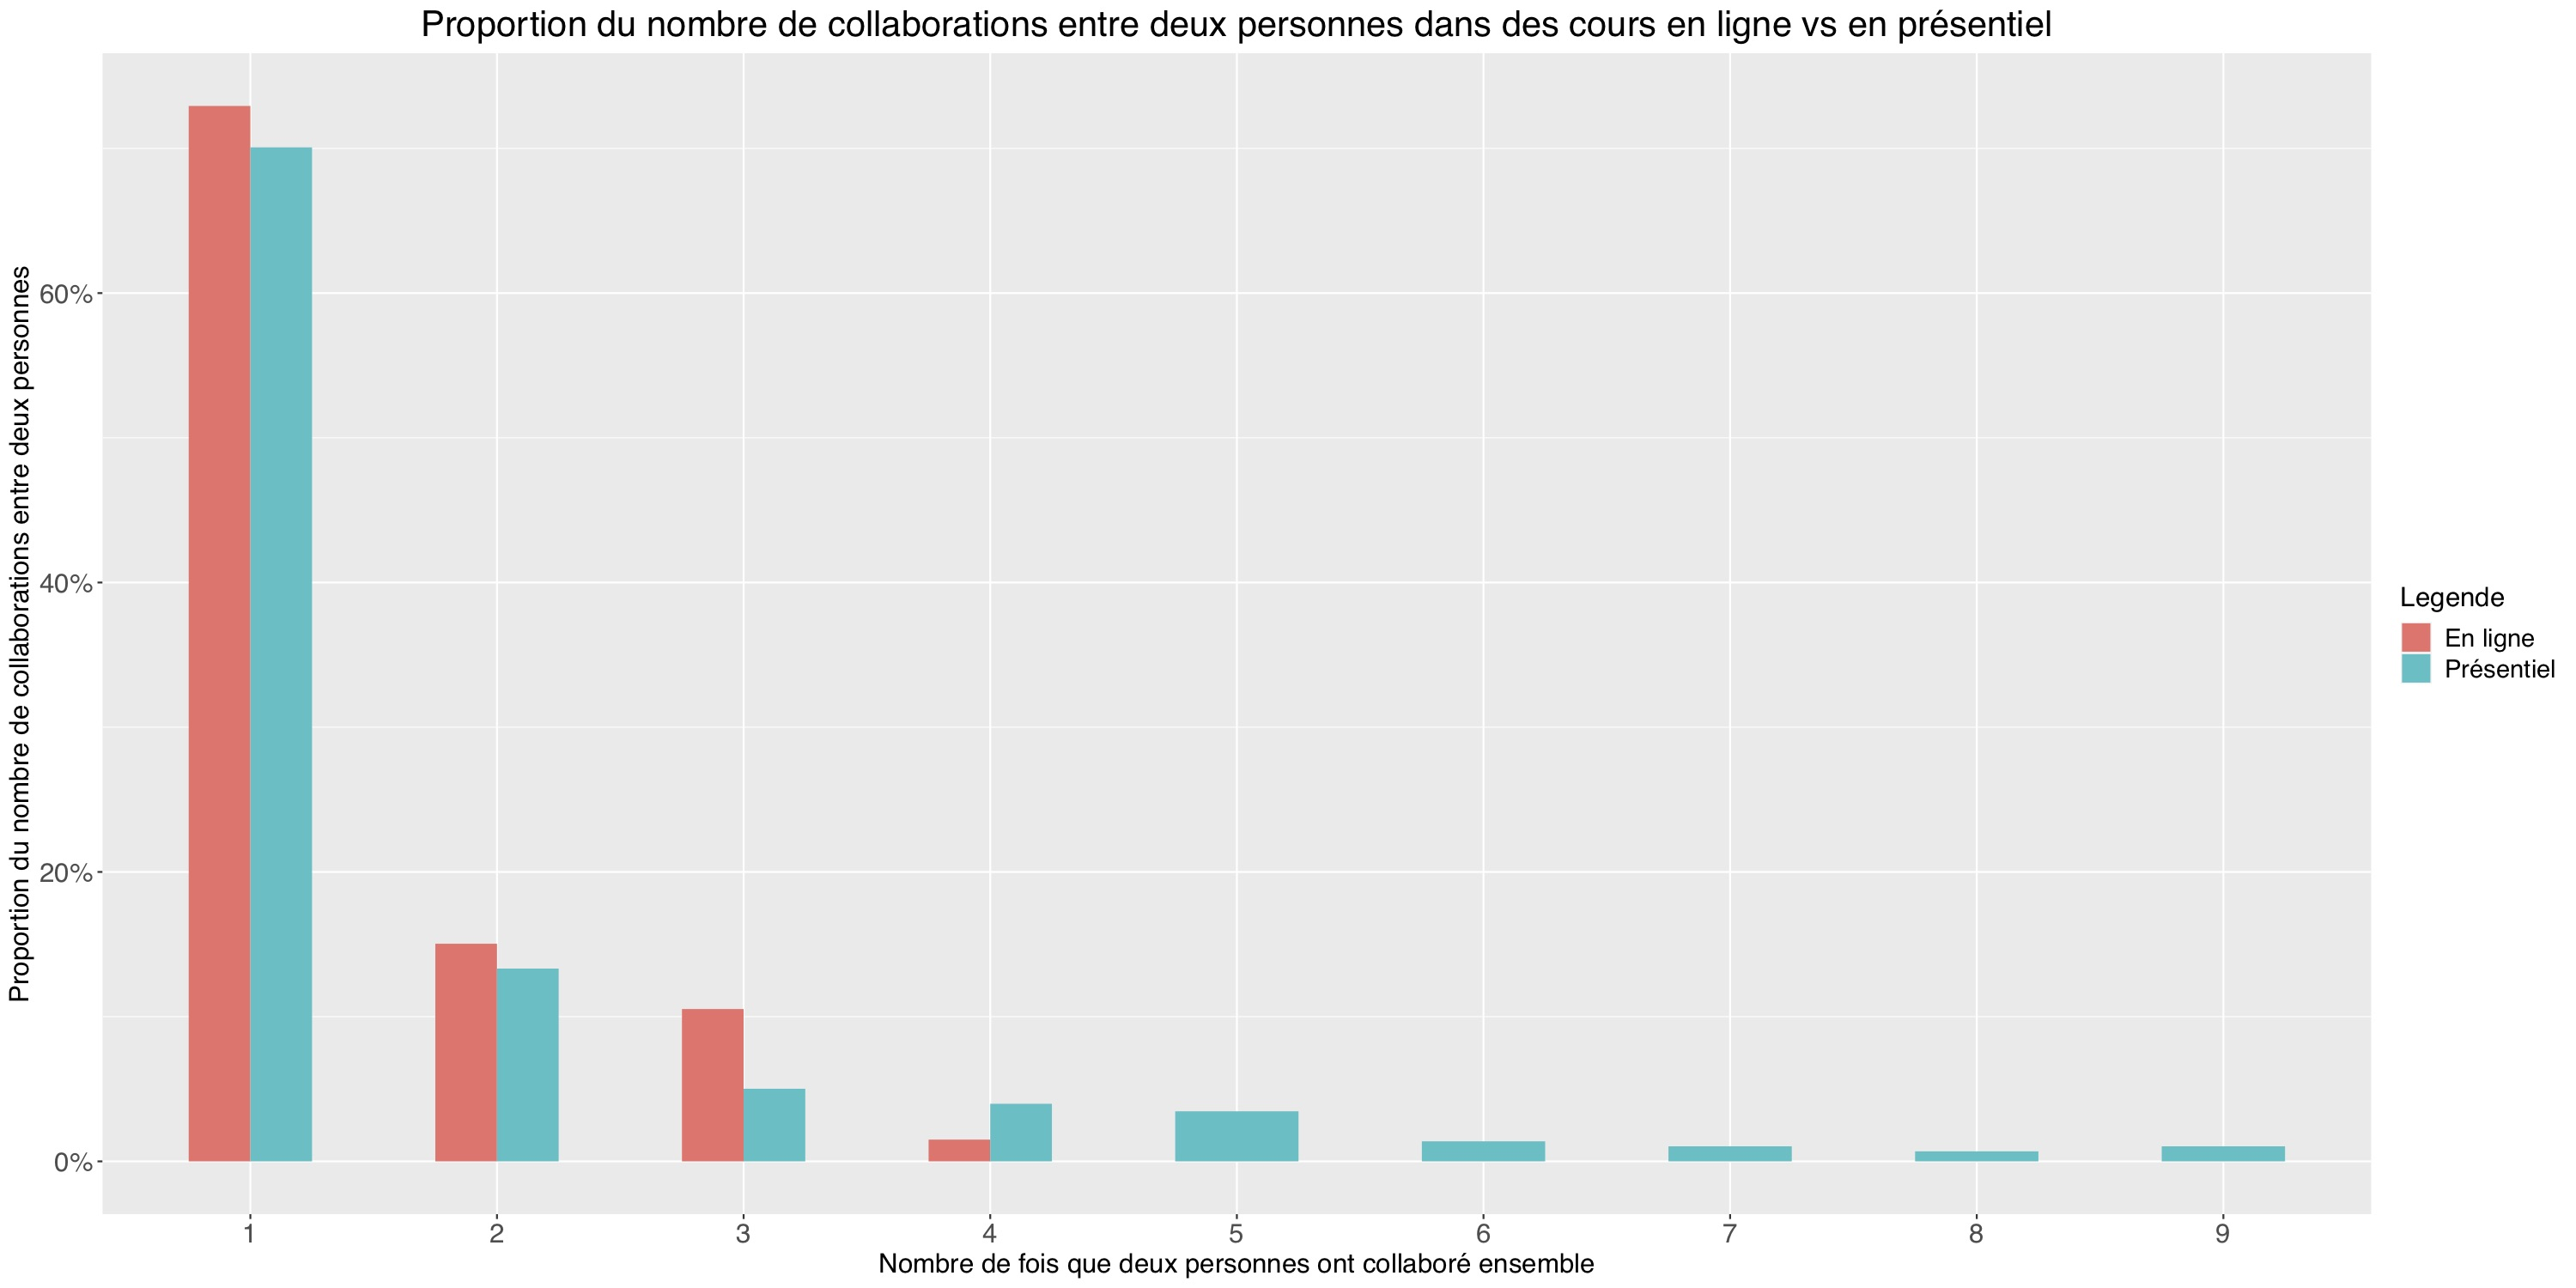
\includegraphics[scale=0.15]{Histogramme3.jpg}}
\caption{Histogramme de comparaison des proportions du nombre de fois qu'il y a eu collaboration avec les mêmes personnes entre les cours en ligne et en présentiel.}
\label{fig}
\end{figure}

\section{Discussion}
Dans le tableau 1, la moyenne plus basse du nombre de collaborations par étudiant dans la période post-Covid permet de supposer qu'il y aurait eu moins de travaux d'équipe ou que ceux-ci requéraient des équipes de plus petite taille dans la période post-Covid. De plus, la comparaison des réseaux nous permet d'établir qu'il y a moins de personnes qui font partie du réseau depuis le début de la pandémie. Cet effet n'est toutefois pas nécessairement lié à la Covid. En effet, il est possible que cela illustre le fait qu'à mesure que nous avançons dans le baccalauréat, les cours sont de plus en plus spécialisés et ils sont de moins en moins de type tronc commun entre les différentes concentration du baccalauréat en biologie. Il en résulte alors que les étudiants des concentrations autres qu'en écologie ne sont généralement plus dans les cours des étudiants échantillonnés, soit ceux en BIO500. Donc, la figure 1 et le tableau 1 permettent de comprendre que, dans la période de pandémie, le réseau de collaborations comprend moins de personnes et que ces collaborations sont moins nombreuses. Toutefois, ces effets, bien que probablement significatifs, ne sont pas forcément dûs à la Covid-19.\\[\baselineskip]

Ensuite, la figure 2 nous permet de voir que le choix de coéquipiers est assez varié peu importe la période. En effet, on voit qu'il est bien plus fréquent que les collaborations entre deux personnes aient lieu seulement une fois que plusieurs. Ceci évoque un choix de coéquipier varié la plupart du temps, et ce, indépendamment de la période. Ensuite, il est à noter que dans la figure 3, seulement les cours avec des collaborations (travaux d'équipe) ont été considérés. Ainsi, comme les cours au début du baccalauréat en biologie sont davantage des cours théoriques avec comme seules évaluations des examens individuels, il y a peu de collaborations dans les premières sessions du baccalauréat et donc peu de cours considérés. Comme la période pré-Covid inclus ces premières sessions, il y a moins de cours considérés dans celle-ci. Dans cette figure, même si le nombre total de cours post-Covid est plus grand, cette période comprend une plus grande proportion de cours en ligne. Toutefois, on voit que le fait que les cours se déroulent en ligne ou non n'a pas vraiment d'impact sur le choix de coéquipier. En effet, dans la figure 4 on remarque une tendance similaire dans les deux types de cours soit que la proportion du nombre de collaborations diminue à mesure que le nombre de collaborations entre deux mêmes personnes augmente. Dans les figures 2 et 4, le fait que la catégorie dominante soit celle où il n'y a eu qu'une collaboration par groupe de deux personnes nous permet d'illustrer que les étudiants continuent d'être très variés dans leur choix de coéquipier peu importe le type de cours et la période (pré ou post-Covid). Ceci peut s'expliquer par le fait qu'au fil de notre parcours universitaire, nous apprenons à connaître davantage de personnes dans notre programme. Ainsi, le choix des personnes avec qui nous travaillons peut être plus varié. Également, plus nos études progressent, plus il y a de choix de cours. Cela implique que les gens avec qui les étudiants font équipe habituellement ne se retrouvent pas nécessairement dans les mêmes cours. Cet élément peut augmenter l'ampleur des cercles de collaborations et expliquer que la catégorie dominante soit celle où il n'y a eu qu'une collaboration entre deux personnes. En outre, ces phénomènes semblent avoir eu plus d'impact sur l'appariement des étudiants que les changements liés à la pandémie. D'ailleurs, le choix des étudiants d'opter pour des coéquipiers variés est un choix bénéfique pour ceux-ci, puisqu'il permettrait d'agrandir leur réseau social et, par le fait même, d'améliorer leurs performances académiques \cite{rizzuto_its_nodate}.\\[\baselineskip]

En conclusion, nous ne sommes pas en mesure de confirmer les hypothèses que nous avions concernant l'appariement des étudiants. En effet, le choix conservateur ou non des étudiants et la diversité des équipes ne semblent pas être particulièrement affectés par la pandémie selon nos données. Nous pouvons simplement confirmer que le nombre de cours en ligne a augmenté depuis le début de la pandémie. Dans le futur, il serait intéressant de faire le même exercice avec des étudiants qui ont commencé leur baccalauréat en ligne dans le contexte pandémique et qui sont de retour en présentiel lorsque la pandémie sera terminée. Ainsi, le fait d'avoir connu certains coéquipiers en présentiel au préalable n'influencerait pas les résultats comme nous avons pu le remarquer ici.
\bibliographystyle{plain}
\bibliography{BIO500REF}

\end{document}
